\documentclass[11pt]{scrartcl}
\usepackage{graphicx}
\graphicspath{{./}}
\usepackage[sexy]{evan}
\usepackage[normalem]{ulem}
\usepackage{hyperref}
\usepackage{mathtools}
\hypersetup{
    colorlinks=true,
    linkcolor=blue,
    filecolor=magenta,      
    urlcolor=cyan,
    pdfpagemode=FullScreen,
    }

\renewcommand{\dangle}{\measuredangle}

\renewcommand{\baselinestretch}{1.5}

\addtolength{\oddsidemargin}{-0.4in}
\addtolength{\evensidemargin}{-0.4in}
\addtolength{\textwidth}{0.8in}
% \addtolength{\topmargin}{-0.2in}
% \addtolength{\textheight}{1in} 


\setlength{\parindent}{0pt}

\usepackage{pgfplots}
\pgfplotsset{compat=1.15}
\usepackage{mathrsfs}
\usetikzlibrary{arrows}

\usepackage[most]{tcolorbox}

\begin{document}
    \title{Average}
    \date{G3-4 | \today}
    \author{Azzam (IG:haxuv.world)}
    \maketitle

\section{Quick Notes}
\subsection{Mean / Average}
    Mean is the sum of all numbers (or data) divided by how many the numbers we have.
    \begin{itemize}
        \item For example, the mean of the numbers 3, 5, 7, and 9 is:
\[
\frac{3 + 5 + 7 + 9}{4} = \frac{24}{4} = 6
\]
    \end{itemize}


\subsection{Median}
    Median is the "middle" number. Make sure you order the numbers before count up the median (sort in ascending order). What if there is no middle? (like in 1 2 3 4) Just take the mean between the "left middle" and "right middle".\\
    \textbf{The complete definition:}
\begin{itemize}
    \item The median of a set of numbers is the middle value when the numbers are arranged in order from smallest to largest. For example, the median of the set $\{5, 3, 11, 9, 7\}$ is 7 since it is the middle value when the numbers are arranged as $\{3, 5, 7, 9, 11\}$.

    \item If there are an even number of values, the median is the average of the two middle values. For example, the median of the set $\{3, 5, 7, 9\}$ is $\frac{5 + 7}{2} = 6$ since there are two middle values, 5 and 7.
\end{itemize}

\newpage
\subsection{Mode}
    Mode, is the most frequent, the ones that appear the most. What if there are more than one numbers appear most frequent? We take them all as the mode.

    \textbf{The complete definition:}
\begin{itemize}
    \item The mode of a set of numbers is the value that appears most frequently. For example, the mode of the set $\{3, 5, 7, 5, 9, 5, 11\}$ is 5 since it appears three times, which is more than any other value.

    \item If no value appears more than once, the set has no mode. If two or more values appear the same number of times, the set has multiple modes.
\end{itemize}
    
\section{Problems}
\subsection{Warm Up}
\begin{enumerate}
    \item Determine the mean of these numbers: 
    \begin{tcolorbox}[colback=green!10!white,colframe=green!75!black,box align=center,
            halign=center,
            valign=center]
            $1,3,5,7,9$.
        \end{tcolorbox}
        
    \vspace{7.5cm} \item Determine the average of these numbers (don't calculate one by one):
        \begin{tcolorbox}[colback=blue!10!white,colframe=blue!75!black,box align=center,
            halign=center,
            valign=center]
             $1,2,3,4,5,\dots,18,19,20$
        \end{tcolorbox}
        
    \vspace{7.5cm} \item Determine the median of these numbers: 
        \begin{tcolorbox}[colback=green!10!white,colframe=green!75!black,box align=center,
                halign=center,
                valign=center]
                 $6,2,10,3,7,1,1$.
        \end{tcolorbox}
        
    \vspace{7.5cm} \item Determine the median of these numbers: 
        \begin{tcolorbox}[colback=red!10!white,colframe=red!75!black,box align=center,
                halign=center,
                valign=center]
                 $7,3,11,4,8,2$.
        \end{tcolorbox}
        
    \vspace{7.5cm} \item What is the mode of these numbers?
        \begin{tcolorbox}[colback=green!10!white,colframe=green!75!black,box align=center,
            halign=center,
            valign=center]
            6  3  3  5  7  4  3  3  1  3  4  7  4  6
        \end{tcolorbox}
    
    \vspace{7.5cm} \item What is the mode of these numbers?
        \begin{tcolorbox}[colback=red!10!white,colframe=red!75!black,box align=center,
            halign=center,
            valign=center]
            4 6  3  5  7  4  3  3  1  3  4  7  4  6
        \end{tcolorbox}

    \vspace{7.5cm} \item What is the mode of these numbers?
        \begin{tcolorbox}[colback=blue!10!white,colframe=blue!75!black,box align=center,
            halign=center,
            valign=center]
            1 2 3 4 5 6 7 8 9 10
        \end{tcolorbox}
    
    \vspace{7.5cm} \item Given 15 integer numbers below. After the largest number and the smallest number are deleted, the average number of the 13 remaining numbers is larger than 4.3 yet smaller than 4.4. What is the value of $x$?
        \begin{tcolorbox}[colback=green!10!white,colframe=green!75!black,box align=center,
        halign=center,
        valign=center]
        6  3  3  5  7  4  $x$  3  3  1  3  4  7  4  6
        \end{tcolorbox}

    \vspace{7.5cm} \item For the 13 numbers below, the median is $y$, and the average number is 4. Find $x+y$.   
       \begin{tcolorbox}[colback=red!10!white,colframe=red!75!black,box align=center,
        halign=center,
        valign=center]
        6 3 3 5 1 4 $x$ 3 2 2 9 4 7
        \end{tcolorbox}
\vspace{7.5cm} 
\end{enumerate}

\subsection{Challenges}
\begin{enumerate}[resume]
    \item The average of three numbers is 99. If one of them is increased by 9, the average will increase by \ldots

    \vspace{7.5cm} \item Given three positive numbers with median = mean = $x$.After the median is erased, we calculate the new average $y$. What is $\frac{x}{y}$?
    
    \vspace{7.5cm} \item In a math quiz, Ali scored 15 points less than Ben, who scored 95 points. Chloe scored half as many points as Ali. What is their mean score?

    \vspace{7.5cm} \item Given 7 integers. Their mean, median, the only mode, and range are all 7. Among these 7 integers, which option below cannot be the smallest number?
    \begin{enumerate}
       \item[(A)] 2
       \item[(B)] 4
       \item[(C)] 5
       \item[(D)] 6
   \end{enumerate}


    \vspace{7.5cm} \item Given that 5 workers have to pave a 6km 30m long road in 6 days. How many meters of the road should be done in a day on average?

    \vspace{7.5cm} \item Suppose the 7 numbers given are 3, 2, 5, 5, 6, 2, and 5. If another number 4 is given, which statistic will change?
    
    \vspace{7.5cm} \item Below is the math test result of a class of 41 students. Find the median and mode of their scores.\\
        \begin{tabular}{c|cccccc}
            \hline
            Score & 50 & 60 & 70 & 80 & 90 & 100\\
            \hline
            Number of People & 1 & 12 & 8 & 13 & 4 & 3\\
            \hline
        \end{tabular}

     \vspace{7.5cm} \item The line graph shows the five baseball teams that the boys and girls in Jeff's class support. Find the team which has the most supporters and the team with the median of the numbers of supporters.
    
        \begin{center}
            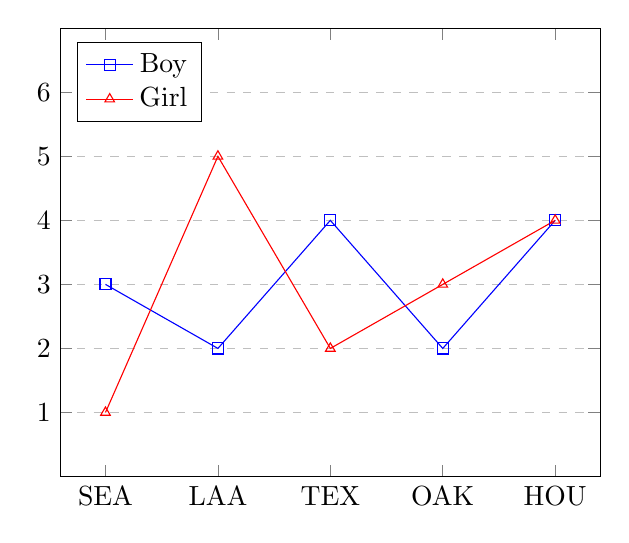
\begin{tikzpicture}
                \begin{axis}[
                    xlabel={},
                    ylabel={},
                    xtick=data,
                    xticklabels={SEA,LAA,TEX,OAK,HOU},
                    ytick={1,2,3,4,5,6},
                    ymin=0,ymax=7,
                    legend pos=north west,
                    ymajorgrids=true,
                    grid style=dashed,
                ]
                \addplot[color=blue,mark=square,]
                    coordinates {(0,3)(1,2)(2,4)(3,2)(4,4)};
                \addplot[color=red,mark=triangle,]
                    coordinates {(0,1)(1,5)(2,2)(3,3)(4,4)};
                \legend{Boy,Girl}
                \end{axis}
            \end{tikzpicture}
        \end{center}

    \vspace{7.5cm} \item The record shows the national football clubs that had won the Europe championship for the last 50 years. Which country does the median of the numbers of times of championship fall on?
    \vspace{\baselineskip}
    \begin{tabular}{cc|cc|cc|cc|cc}
        \hline\hline
        73 & Netherland & 83 & Germany & 93 & France & 03 & Italy & 13 & Germany\\
        74 & Germany & 84 & England & 94 & Italy & 04 & Portugal & 14 & Spain\\
        75 & Germany & 85 & Italy & 95 & Netherland & 05 & England & 15 & Spain\\
        76 & Germany & 86 & Romania & 96 & Italy & 06 & Spain & 16 & Spain\\
        77 & England & 87 & Portugal & 97 & Germany & 07 & Italy & 17 & Spain\\
        78 & England & 88 & Netherland & 98 & Spain & 08 & England & 18 & Spain\\
        79 & England & 89 & Italy & 99 & England & 09 & Spain & 19 & England\\
        80 & England & 90 & Italy & 00 & Spain & 10 & Italy & 20 & Germany\\
        81 & England & 91 & Serbia & 01 & Germany & 11 & Spain & 21 & England\\
        82 & England & 92 & Spain & 02 & Spain & 12 & England & 22 & Spain\\
    \hline\hline
    \end{tabular}


\end{enumerate}
\end{document}